%!TEX root = main.tex
\section{Einführung}
		
	\begin{minipage}[t][\textheight][t]{0.7\textwidth}
	Der wesentliche Gegenstand dieser Arbeit, ist die Veröffentlichung "The Alexander Polynomial of a 3-manifold and the Thurston norm on cohomology" von McMullen~\cite{McMullen2002}. 

    In dem Fall, dass eine gegebene kompakte 3-Mannigfaltigkeit homöomorph zu einem Knotenkomplement ist --- genauer gesagt, zu einer Sphäre aus der eine offene Tubenumgebung eines eingebetteten Knotens entfernt wird --- ist der Rang der Fundamentalgruppe 1, also $b_1(M)=1$. Das genauere Studium der Fundamentalgruppe erweist sich als schwierig, deswegen geht man zu der Abelianisierung der Kommutatoruntergruppe über. Diese ist nach Hurewicz isomorph zu der ersten Homologiegruppe der zyklischen Überlagerung. Da aber auch diese Gruppe im Allgemeinen nicht endlich erzeugt oder endlich präsentiert ist, betrachtet man die induzierte Wirkung der Decktransformationen auf der Homologie, weiter betrachtet man sogar die Wirkung des Gruppenrings $\ZZ [t^{\pm 1}]$, wobei $t$ Erzeuger der Deckgruppe ist, die aus der abelschen Gruppe einen $\ZZ [t^{\pm 1}]$-Modul macht --- den Alexander Modul. 
    Der Alexander Modul zeichnet sich durch weniger Erzeuger und Relationen aus und bietet eine fruchtbare Grundlage für algebraische Invarianten, inspieriert durch die Knotentheorie. Genau diese Inspiration liegt dem Paper von McMullen zu Grunde. Er verallgemeinert darin eine Abschätzung zweier Invarianten (auf Knotenkomplementen) aus der Knotentheorie, auf allgemeinere Klassen von 3-Mannigfaltigkeiten.

	\vfill
	\begin{minipage}[t]{0.7\textwidth}
		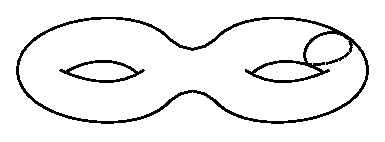
\includegraphics{zyklbott} 
	\end{minipage}
	\begin{minipage}[t]{0.2\textwidth}
	\vspace{-1cm}
	$\longrightarrow$
	\vfill
	\end{minipage}
	\vspace{1.5cm}
	\end{minipage}
	\begin{minipage}[t]{0.3\textwidth}
	\vfill
	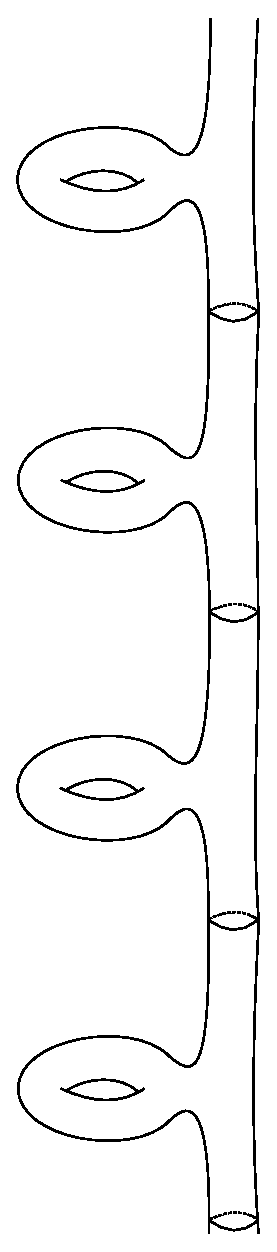
\includegraphics{zyklright} 
	\end{minipage}
    

    Bei der Alexander-Norm eines Homomorphismus in $\Hom(\pi_1(M),\ZZ)$ handelt es sich um den Grad des zugehörigen Alexander Polynoms und die Thurston-Norm weist einem solchen Homomorphismus die minimale Komplexität einer Poincaré-Lefschetz dualen eingebetteten Fläche zu. Ohne die genauere Definition hier zu nennen, soll nun das Theorem vorgestellt werden, dessen Beweis in dieser Arbeit behandelt wird.
    \begin{thm}[McMullen]
    \label{thm:haupttheorem}
    	Sei $M$ eine kompakte, zusammenhängende, orientierbare Mannigfaltigkeit der Dimension 3. Falls der Rand dieser Mannigfaltigkeit nicht leer ist, so soll er aus einer Kollektion von Tori bestehen. Dann gilt folgende Abschätzung für die Alexander-Norm und die Thurston-Norm $\alex \cdot ,\thur \cdot : H^1(M;\ZZ) \to \RR$ der 3-Mannigfaltigkeit:
    	\[
    		\alex \phi \leq 
    		\begin{cases}
    			\thur \phi + 1+ b_3(M) &\text{, falls } b_1(M)\leq 1 \text{ und } \phi: \pi_1(M) \onto \ZZ \\
    			\thur \phi &
    		\end{cases}
    	\]
    	Ist $\phi$ von einer Faserung $M\to S^1$ induziert, so gilt Gleichheit.
    \end{thm}